% article document class appropriate for small (<100 pages) documents
\documentclass{article}

% Packages provide additional functionality
\usepackage{url}
\usepackage{graphicx}
\usepackage{subfig}
\usepackage{float}
\usepackage{listings}
\usepackage{color}
\usepackage{enumitem}
\usepackage{amsmath}

\newcommand{\sa}{s\alpha}
\newcommand{\ca}{c\alpha}
\renewcommand{\sb}{s\beta}
\newcommand{\cb}{c\beta}
\newcommand{\sg}{s\gamma}
\newcommand{\cg}{c\gamma}

\title{Assignment in RobWork and Euler angles}
\author{Martin Toft Franzen, Martin Moghadam, Robertas Jacauskas,\\
 Audrius Palisaitis and Kalle Grafstr�m}

\begin{document}

\maketitle % reads info from \title and \author above

% auto-generated from previous compilation pass, you may need to run
% latex twice to get up-to-date table of contents
%\tableofcontents

% Intro section
\section{Introduction}

The report documents the project of subtask 5 in the course RSD, Robot System Design.

\subsection{Project Description}

The the beginning of the course we were handed a description of subtask 5:

\begin{itemize}
\item Task description
	\begin{itemize}
	\item Everybody knows that washing black and white together is a bad idea, but there are a lot more criteria to consider, to prepare a wash
		\begin{itemize}
		\item Appropriate colors for joint was
		\item Washing conditions - e.g. temperature, centrifugation, spinning speed, drying
		\end{itemize}
	\item The appropriate amount of laundry should be prepared in piles or containers, which correspond to the load size of a washing machine
	\item When elders move in their clothes will be tagged (subtask 6), but the washing recipes of each item should also be registered
		\begin{itemize}
		\item That task should be simple for the staff
		\end{itemize}
	\end{itemize}
\item Challenges
	\begin{itemize}
	\item Together with group of subtask 6 create an easy an appropriateinterface for registering clothes and washing recipes
	\item Control criteria for the robot arm in subtask 4
	\item Close collaboration with subtask 4 and 6
	\item Perhaps some “untagged” clothes shouldbe put in washing bags?
	\end{itemize}
\item Technologies available
	\begin{itemize}
	\item ???
	\end{itemize}
\end{itemize}

The description explains the task, the challenges the task poses and that we should investigate the technologies available.

\subsection{Structure of System}
\section{Calculations}
\label{sec:calc}
The Rotation matrices for the 24 common Euler and fixed angleset conventions are all defined in appendix B in the course book\cite{bib1}. These can be used directly to calculate the rotation matrices for a given angleset based on three input angles. The equations for calculating the angles based on the rotation matrix are not documented fully in the book however.\\

An example of how to derive these equations are shown below. This example is based on the  angleset Euler XYZ shown in equation \eqref{eq:eq0}. 

\begin{equation}
R_{{X^I}{Y^I}{Z^I}}(\alpha,\beta,\gamma) =
\begin{bmatrix}
\cb \cg & -\cb \sg & \sb \\
\sa \sb \cg + \ca \sg & -\sa \sb \sg + \ca \cg & -\sa \cb \\
-\ca \sb \cg + \sa \sg & \ca \sb \sg + \sa \cg & \ca \cb
\end{bmatrix}
\label{eq:eq0}
\end{equation}


The input angles are found according to equation \eqref{eq:eq1}, \eqref{eq:eq2} and \eqref{eq:eq3} by using the atan2-function.
\begin{align}
\beta  &= Atan2(sin(\beta ),cos(\beta ))   \label{eq:eq1} \\
\alpha &= Atan2(sin(\alpha ),cos(\alpha )) \label{eq:eq2} \\
\gamma &= Atan2(sin(\gamma ),cos(\gamma )) \label{eq:eq3}
\end{align}

The Atan2-function takes two parameters, namely the sine and cosine element of a variable. From equation \eqref{eq:eq1} the sine part of $\beta$ is derived as shown in equation \eqref{eq:eq4} and the cosine part in equation \eqref{eq:eq5}.

\begin{equation}
sin(\beta )=r_{13}
\label{eq:eq4}
\end{equation}
\begin{equation}
cos(\beta )=\sqrt{r{_{11}}^{2} + r{_{12}}^{2}}
\label{eq:eq5}
\end{equation}

This is derived as shown in equation \eqref{eq:eq6} and makes it possible to rewrite equation \eqref{eq:eq1} to equation \eqref{eq:eq7}.

\begin{align}
r{_{11}}^{2} + r{_{12}}^{2} &= cos(\beta )^2cos(\gamma )^2+cos(\beta )^2sin(\gamma )^2 \nonumber \\
 &=cos(\beta )^2(cos(\gamma )^2+sin(\gamma )^2) \nonumber \\
 &=cos(\beta )^2 \label{eq:eq6}
\end{align}

\begin{equation}
\beta = Atan2(r_{13,\sqrt{r{_{11}}^{2} + r{_{12}}^{2}}})
\label{eq:eq7}
\end{equation}


Solving $cos(\beta)$ makes it possible to solve equation \eqref{eq:eq3} and \eqref{eq:eq4} in an equal manner:

\begin{align}
sin(\alpha ) &= \tfrac{-r_{23}}{cos(\beta )} \nonumber \\
cos(\alpha ) &= \tfrac{r_{33}}{cos(\beta )}  \nonumber \\
\alpha &= Atan2(\tfrac{-r_{23}}{cos(\beta )},\tfrac{r_{33}}{cos(\beta )}) \label{eq:eq10}
\end{align}

\begin{align}
sin(\gamma ) &=\tfrac{-r_{12}}{cos(\beta )} \nonumber \\
cos(\gamma ) &= \tfrac{r_{11}}{cos(\beta )} \nonumber \\
\gamma &= Atan2(\tfrac{-r_{12}}{cos(\beta )},\tfrac{r_{11}}{cos(\beta )}) \label{eq:eq13}
\end{align}

As equation \eqref{eq:eq10} and \eqref{eq:eq13} divides by $cos(\beta)$, having $\beta$ at angles equal to $-90^{\circ}$ or $90^{\circ}$ makes it impossible to derive $\alpha$ and $\gamma$ with these equations. In these cases $\alpha$ is chosen to $0^{\circ}$ making it possible to solve all angles as shown in equation \eqref{eq:eq14} and \eqref{eq:eq15}.

\begin{align}
\beta &= -90^{\circ} \nonumber \\
\alpha &= 0          \nonumber \\
\gamma &= Atan2(-r_{32},r_{31}) \label{eq:eq14}
\end{align}

\begin{align}
\beta &= 90^{\circ} \nonumber \\
\alpha &= 0         \nonumber \\
\gamma &= Atan2(r_{32},-r_{31}) \label{eq:eq15}
\end{align}


The above special cases are an example of equations using $cos(\beta)$. All the conventions can be solved in a similar manner, though some of them uses $sin(\beta)$ to solve $\alpha$ and $\gamma$ angles. In these, the special cases are at $\beta$ angles of $0^{\circ}$ or $180^{\circ}$.\\
Moreover, the Euler XYZ angleset convention is equal to the Fixed ZYX angleset convention. This holds true for all Euler and Fixed anglesets, thus reducing the 24 conventions to 12 unique. Our program solves 6 of these as shown in table \ref{tab:anglesets}.

\begin{table}[H]%
\centering
\begin{tabular}{|c|c|}
\hline
Euler ZYX & Fixed XYZ \\
\hline
Euler XYZ & Fixed ZYX \\
\hline
Euler XZY & Fixed YZX \\
\hline
Euler YXZ & Fixed ZXY \\
\hline
Euler ZXZ & Fixed ZXZ \\
\hline
Euler ZYZ & Fixed ZYZ \\
\hline
\end{tabular}
\caption{Implemented angleset conventions}
\label{tab:anglesets}
\end{table}

%\begin{figure}[H]
%  \centering
%  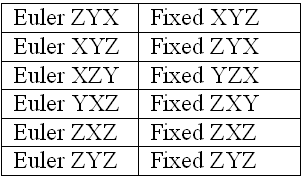
\includegraphics[scale=0.5]{tex/figure_17.png} 
%  \caption{}
%  \label{fig:table1}
%\end{figure}

\section{RobworkStudio plugin}
\label{sec:plugin}
In addition to the Letter Font application a plugin for RobworkStudio has been created. The purpose of this plugin is to read Cartesian coordinates from a file similar to the one created by the Letter Font program and then output both a RobworkStudio simulation file and a jnt-file for direct use with the Fanuc robot. In addition to the main functionality the plugin has a button to test the input coordinates, and examine if they correspond with the Farnuc robot workspace and outputs the joint values, the button is called "Test".

\subsection{Parser}
\label{sec:parser}
To parse an input file a list of criteria must be met:
\begin{itemize}
	\item Txt file format. The parser only accepts files with the extension txt, even if the files are written in any form of clear text. 
	\item Letter allocation. Coordinates are allocated into subgroups according to letters. The parser scans for the keyword \textit{Letter = \$} to signify a new group of coordinates allocated to a specific letter. A letter can be any character or number except space.
	\item Letter separation. Letters are separated by the keyword \textit{NEXT\_LETTER} to signify the end of a group.
	\item Coordinate formating. Coordinates must be on individual lines, each component separated by a tabular. Coordinates are assumed to be integer (pixel) values corresponding to millimeter offsets on the individual axes from an origin specified by the plugin based on the selected robot device. The X axis specifies the height of text, 0 and negative being furthest from the robot. The Y axis specifies the width of the text, with 0 and negative to the left of the robot. The Z axis specifies the elevation of the toolhead when milling, with 0 at table level and positive values elevating the drill above it.
	\item Density specification. The toolhead will be lifted with a fixed value when moving between letters. This is to avoid carving connecting paths between them. To enable the plugin to lift the toolhead when milling complex letters or gaps in these, the density of coordinates must be specified in the file with the keyword \textit{Density = \$}. The parser assumes that coordinate density is quadratic and therefore equal on both the X and Y axes.
\end{itemize}

If an input file respects this specification the parser will most likely parse the file successfully.\\

The actual implementation of the parser is described in the following section.

\subsubsection{Implementation}
\label{sec:parserImpl}
The sscanf (formatted string reader) and strstr (locate substring) is used to parse the input file. Which is read by ifstream (input file stream). All parse functionality is C portable, primarily because the programmer was familiar with these functionalities, and the functionality was appropriate for the task.  

\subsection{Path planning and joint angle solving}
\label{sec:pathplanning}
Despite its name, path planning is not a feature that is used at all in the final implementation of the plugin. The functionality is implemented based on the Robworks manual, but the overhead imposed by the planner is considerable and the gain was deemed insignificant in the end since mostly all coordinates are inside the target milling material and therefore either always or never collides with an object. In addition the paths between these coordinates are generally short and trivial, rendering the pathPlanner unnecessary. A function called \textit{pathPlanner} exists in the project namespace but is never used and is only provided as an addon for future use.\\

The main part of the plugin handles the conversion from the parsed Cartesian coordinates into rotation values for each of the robots joints. These are determined by using inverse kinematics (henceforth written as IK). More specifically, one of the inbuilt iterative IK solvers called ResolvedRateSolver is used through the IK wrapper IKMetaSolver. The values are then stored in a vector array of configurations. This array is passed to a function that converts each configuration into a joint parameter configuration and printed to the output jnt file.

\subsubsection{Implementation}
\label{sec:pathplanningImpl}



% Conclusion
\section{Conclusion}



\nocite{bib1} % Creates entry in bibliography even if it isn't cited.


\addcontentsline{toc}{section}{References} % Include references in TOC
\bibliographystyle{unsrt} % references appear in order of citations
\bibliography{references}


\end{document}